\chapter{Basic Concepts and Terms}%
\label{basicConcepts}
%\section{Basic Concepts}
    In this chapter, the foundation for exploring the subject matter is laid by introducing the fundamental concepts and key terminology that will form the basis of this thesis.
    This section defines relevant terms and provides background information on task mapping, communication message routing, time-triggered scheduling, automotive safety standards, vehicle communication protocols, safety-related requirements in vehicle E/E architecture, design space exploration, and virtualization technology.




\section{Task Mapping or Resource Allocation}

%Allocation of the tasks in the multi-core can be performed in design-time or run-time. There is no application running during design-time task allocation as opposed to run-time mapping, where the tasks can be assigned to different cores, while the system is running. When the application requirements are fairly deterministic, design-time mapping is preferred, whereas the run-time assignment should be used when the application requirements are changing in dynamic scenarios and there is a need for reassignment. 
    Multi-core architecture can be classified into two categories, homogeneous and heterogeneous, based on the application's and user's specific needs and requirements. In the homogeneous multi-core architecture, all cores are the same, possessing similar computing capacity and instruction set architecture (ISA). On the other hand, heterogeneous architecture comprises a combination of different cores, each specifically designed to meet particular needs, such as high performance or low power consumption~\cite{gupta2021mapping}.
%Various types of processing units can be integrated on a single chip by utilizing heterogeneous architecture, which ensures lower energy consumption and better flexibility~\cite{singh2013mapping}. Besides, automotive applications increase the demand for heterogeneous architecture because of different contexts and needs. In terms of task mapping complexity, a homogeneous processor requires less work than a heterogeneous one since it has identical cores. Furthermore, homogeneous multi-cores do not need task analysis based on core properties for task execution in contrast to heterogeneous multi-core architecture.
    Integrating multiple types of processing units onto a single chip through heterogeneous architecture results in lower energy consumption and increased flexibility~\cite{singh2013mapping}. This approach is beneficial for automotive applications that have varying contexts and requirements. However, it is essential to note that homogeneous processors require less task mapping complexity than heterogeneous processors, as they have identical cores. Furthermore, homogeneous multi-cores do not require an analysis of core properties for task execution, unlike heterogeneous multi-core architecture.

    The allocation of tasks in a multi-core system can occur either during design-time or run-time. Design-time task allocation is performed when no application is running, in contrast to run-time mapping, which allows tasks to be assigned to different cores while the system is in operation. In cases where the application requirements are predictable and stable, design-time mapping is favored. However, the run-time assignment should be utilized when the application requirements are subject to change in dynamic scenarios, and there is a requirement for reassignment~\cite{askaripoor2022architecture,askaripoor2023designer}.



    Design-time mapping is preferably utilized when the application requirements are fairly deterministic. On the other hand, in case of changes in the requirements in dynamic scenarios, the run-time assignment is preferred because reassignment is required.
    Static mapping uses all system information (e.g., hardware and
    application properties) to find the optimal solution. In addition, this type of mapping is
    appropriate when there is a set of predefined requirements for the applications and hardware. In other words, the design-time methodology cannot solve the mapping problem dynamically. Higher quality solutions can be obtained with the design-time mapping rather than the run-time allocation due to less limitation of the computational power~\cite{askaripoor2022architecture, askaripoor2023designer}. Figure~\ref{fig21} shows the static mapping of several applications, each including threads with different periods and execution times, to an HPCU comprising six cores.



\begin{figure}[t]
\centering
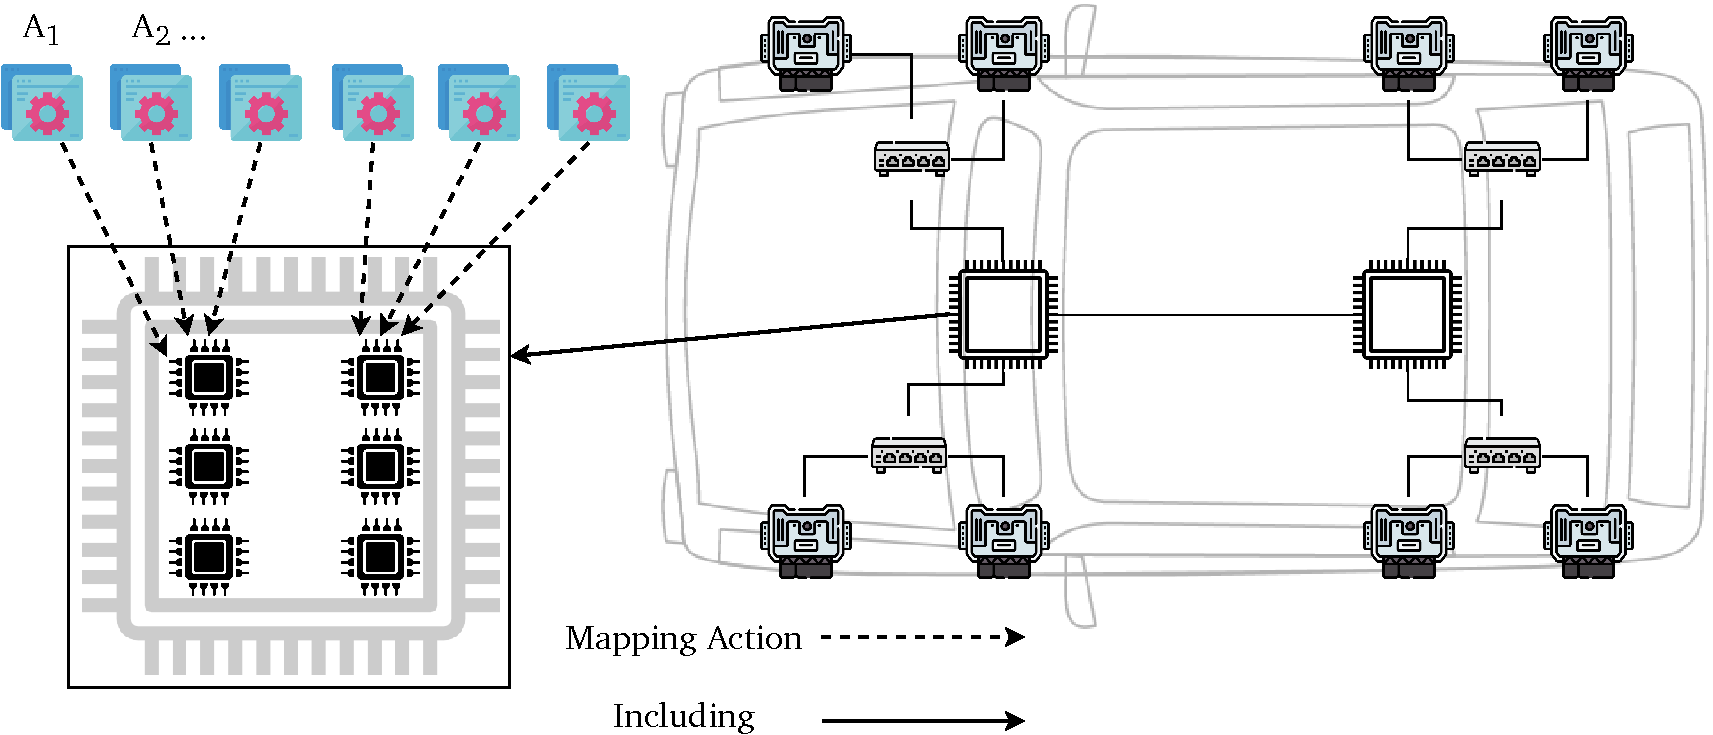
\includegraphics[width=1\textwidth]{figures/mappingaction.pdf}
\caption{Assignment of applications to an HPCU consisting of six cores. }
\label{fig21}
\end{figure}


    \section{Time-triggered Scheduling}\label{TT_Sched}

    In mixed-critical systems, especially those focused on real-time applications, enabling deterministic message delivery (i.e., all computations must be complete before their respective deadlines), avoiding message overlap, and ensuring low latency are extremely important. Scheduling policies help to meet these requirements using various algorithms. Time-triggered scheduling is one of the most common scheduling schemes used in the automotive industry to schedule communication tasks and activities. 
    In the automotive domain, time-triggered scheduling is used in various systems, including engine control, braking, steering, and infotainment. This scheduling scheme also controls safety systems, such as airbags and seatbelts. These systems must respond quickly and reliably to potential hazards, and this scheduling scheme can ensure that the tasks related to these systems are executed at the appropriate times. It is also used in other real-time and mixed-critical systems, such as aviation and industrial control, where predictability and reliability are critical~\cite{zeng2010schedule,lukasiewycz2012modular,askaripoor2023designer}.



    In this type of scheduling, activities/tasks that are periodic are initiated at predefined times (see Figure~\ref{fig22}). A deterministic scheduling approach ensures that tasks in a system are executed at a predictable and repeatable rate. In other words, everything is scheduled before the system is deployed, and it is known in advance which activity will run and when~\cite{schild2000scheduling}. Moreover, all tasks must not overlap during execution~\cite{zhang2014task}. The running processes in ECUs and HPCUs can be scheduled using the time-triggered method. This policy can be applied to the in-vehicle communication network to schedule communication frames/tasks over a communication protocol, e.g., Ethernet.
    Time-triggered scheduling is often used with other scheduling algorithms, such as event-triggered scheduling, to provide a balance between predictability and flexibility~\cite{zeng2010schedule}. In an event-triggered system, a processing task begins in response to the occurrence of a notable event~\cite{tabuada2007event}. While in a time-triggered system, the activities are initiated periodically at predetermined points in real-time.


%Furthermore, finding the correct schedules become an NP-hard problem as the size of the automotive network increases.  


%An example of calculated time-triggered schedules based on periods, the execution time of threads, and the frame length of communication tasks are depicted in figure~\ref{mapping} (b) and figure~\ref{routing} (a).

%Time-triggered scheduling is a method of organizing the execution of tasks in real-time systems. It is a deterministic scheduling approach that is used to ensure that tasks in a system are executed at a predictable and repeatable rate. This scheduling algorithm specify a schedule of tasks to be executed at fixed intervals or at specific points in time. This scheduling scheme is often implemented using a real-time operating system (RTOS) that provides support for scheduling and synchronization of tasks.~\cite{schild2000scheduling}.
%Time-triggered scheduling is a method of scheduling tasks in real-time systems that is based on the use of fixed, periodic execution times for tasks. 


    To illustrate how time-triggered scheduling works, an example of scheduling four tasks is considered within an automotive real-time operating system (RTOS) running on an HPCU. Each task is specified as $T_i~= $\{$T_i^p, T_i^e$\}, where $T_i^p$ represents the task's period, and $T_i^e$ denotes its execution time. The four periodic tasks are as follows: $T_1=$\{$6, 0.5$\}, $T_2=$\{$6, 1.5$\}, $T_3=$\{$6, 0.8$\}, and $T_4=$\{$12, 2$\}. 
    In the context of time-triggered scheduling, the objective is to ensure that each task executes once within its specified period without overlapping with other tasks. As illustrated in Figure~\ref{fig22}, each task completes within its defined period, e.g., $T_4$ finished its job once within its period, which is 12. The visualized schedules confirm no overlap between task execution slots; this demonstrates the correctness of the task schedules under time-triggered scheduling.




%Therefore, taking the time-triggered scheduling into account, each task must be executed once in its period while it does not overlap with other tasks. According to figure~\ref{fig22}, each task is done once in its period and based on the visualized schedules there is no overlapping between the slots which means having correct schedules for the tasks. 
    In Figure~\ref{fig22}, hyperperiod refers to the least common multiple (LCM) of the periods of all periodic tasks or events in a system. It represents the time interval after which all periodic tasks will simultaneously repeat or hyperperiodically align. It helps to determine the maximum scheduling interval required to ensure that all tasks can be scheduled without deadline violations. When the scheduling interval is set to the hyperperiod, it guarantees that all tasks will complete their cycles within that interval, thus avoiding task deadline misses~\cite{askaripoor2023designer}. In this specific example, the hyperperiod is calculated as $12$, which is the LCM of the periods $T_1$, $T_2$, $T_3$, and $T_4$.  




    \begin{figure}[t]
    \centering
    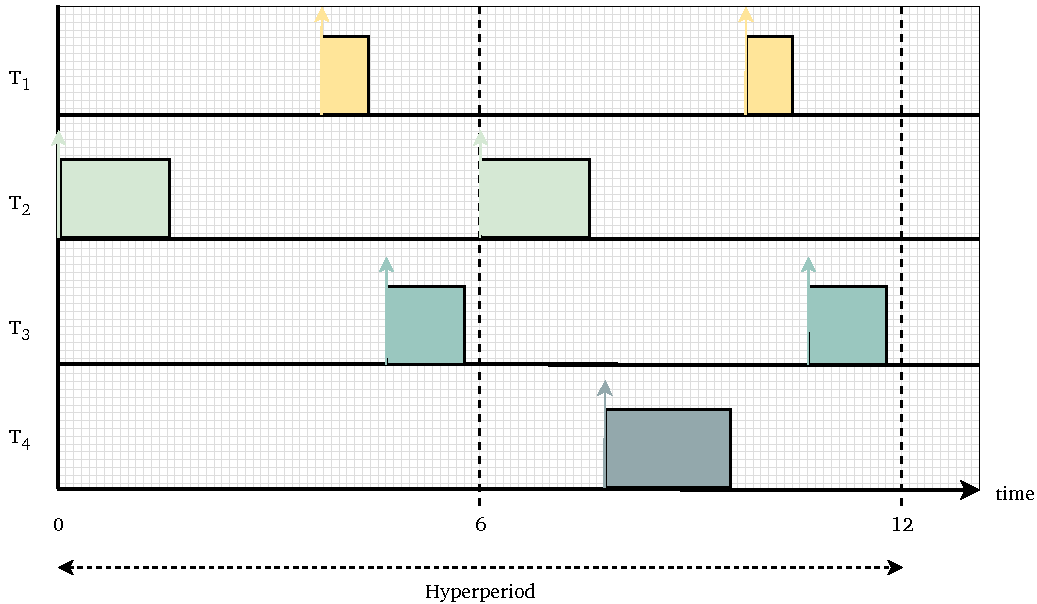
\includegraphics[width=1\textwidth]{figures/timetriggered_v3.pdf}
    \caption{The time-triggered slots of four periodic tasks, namely $T_1$, $T_2$, $T_3$, and $T_4$. An arrow alongside each slot indicates the starting point of the respective task. }
    \label{fig22}
    \end{figure}

%%%%----------------------another exmaple------------------------------------------------
%Imagine that a vehicle has a system for monitoring and maintaining the tire pressure. This system includes sensors that measure the pressure in each tire and a controller that receives the sensor data and processes it. The controller may be programmed to perform certain tasks at specific intervals, such as checking the tire pressure and displaying a warning message if any of the tires are under-inflated.To implement this functionality using time-triggered scheduling, the controller might be programmed to check the tire pressure every 15 minutes, or at some other predetermined interval. When the time arrives for the controller to perform the task, it will retrieve the latest sensor data, process it, and take any necessary actions (such as displaying a warning message). The controller will then wait until the next scheduled time to perform the task again.This type of time-triggered scheduling can be used in a variety of automotive applications to ensure that tasks are performed at regular intervals or at specific points in time. It can be particularly useful in systems that require precise timing or that need to perform tasks even when the vehicle is not in use (such as when the vehicle is parked and the engine is off).

%55-------------------------------------------another example--------------------------

%In the automotive communication domain, time-triggered scheduling is a technique used to ensure that certain tasks are performed at specific intervals or at predetermined points in time. Here is an example of how time-triggered scheduling might be used in an automotive communication application:Imagine that a vehicle has a system for transmitting and receiving data over a wireless communication network. This system includes a controller that processes the data and a wireless interface for transmitting and receiving the data. The controller may be programmed to perform certain tasks at specific intervals, such as sending a status update to a central server or receiving updates from other vehicles on the road.To implement this functionality using time-triggered scheduling, the controller might be programmed to transmit or receive data at predetermined intervals, such as every 5 seconds or every minute. When the time arrives for the controller to perform the task, it will retrieve the data to be transmitted or received, process it, and take any necessary actions (such as sending a status update to a central server or receiving updates from other vehicles). The controller will then wait until the next scheduled time to perform the task again.This type of time-triggered scheduling can be used in a variety of automotive communication applications to ensure that tasks are performed at regular intervals or at specific points in time. It can be particularly useful in systems that require precise timing or that need to perform tasks even when the vehicle is not in use (such as when the vehicle is parked and the engine is off).

    \section{Communication Message Routing}
%-----------------------------------------must be paraphrased--------------------------------
    Message routing plays a crucial role in automotive networks, where many ECUs collaborate to ensure smooth vehicle operations. As modern automobiles become increasingly sophisticated, incorporating various functionalities and advanced systems, efficient and reliable message routing becomes paramount.
    
   \begin{figure}[t]
    \centering
    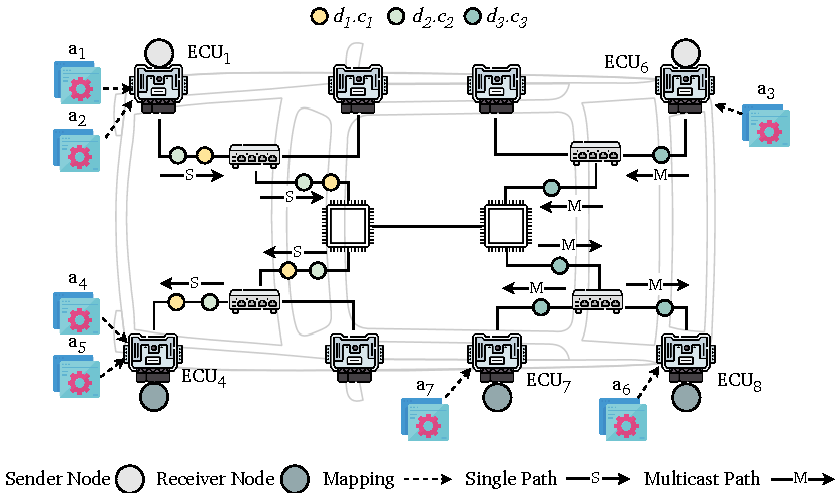
\includegraphics[width=1\textwidth]{figures/routing_basicCon.pdf}
    \caption{Single and multicast routes within a car E/E topology for transferring communication messages from senders to receivers. The communication messages are generated by applications executing on ECUs.}
    \label{fig23}
    \vspace{-8pt}
    \end{figure}
    The ADAS capabilities and new infotainment systems introduce an increasing amount of computational power in control units and data, which needs to be transmitted via an in-car communication network. A valid routing is required in an in-vehicle network to transmit messages from a node (e.g., an ECU) as a sender to another node as a receiver. Due to increasing the size of automotive communication networks, which causes a large number of applications, nodes, and transmitted messages, finding a valid path between two nodes becomes extremely time-consuming and complex because of a significant expansion of the design space~\cite{9565115,smirnov2017optimizing, askaripoor2023designer, 9613692}.
    
    
    One commonly used technique in message routing is the concept of gateways. Gateways act as intermediaries, connecting different network domains or protocols within the vehicle. They receive messages from one network and forward them to another, often performing protocol conversions or message translations. Gateways play a critical role in integrating legacy and newer ones, enabling seamless communication between nodes, e.g., ECUs operating on different protocols. The most essential vehicle communication protocols will be explained in the next section.
    Another essential aspect of message routing is the consideration of real-time constraints. Many automotive applications demand deterministic and timely message delivery to ensure safety and optimal system performance. Therefore, routing algorithms must prioritize critical messages and allocate network resources accordingly. This involves analyzing the network's traffic patterns, identifying potential bottlenecks, and selecting the most efficient paths to ensure timely message delivery and avoid congestions~\cite{askaripoor2023designer,9565115, smirnov2018automatic}.
 
    The framework introduced in this thesis has the capability to create various types of communication message routings, encompassing single, multi-cast, redundant, and homogeneous redundant paths. Detailed descriptions of each type are provided in Chapter~\ref{method}.
    %The introduced framework in this thesis is capable of creating different types of routings for communication messages including single, multi-cast, redundant, and homogeneous redundant paths. The details of each type will be described in Chapter~\ref{method}.
    %Based on the car topology shown in figure~\ref{fig23}, two types of paths from senders to receivers are presented. A single path which transfers two communication messages $d_1$ and  $d_2$ including their tasks, $c_1$ and $c_2$, respectively, from ECU$_1$ as the sender to ECU$_4$ as the receiver. While, the multicast route shows sending a communication message, $d_3$, from a sender, ECU$_6$, to two receivers such as ECU$_7$ and ECU$_8$. 
    Based on the car topology depicted in Figure~\ref{fig23}, two types of communication paths, from senders to receivers, are presented. The single route involves the transfer of two communication messages, $d_1$ and $d_2$, along with their respective tasks, $c_1$ and $c_2$, from ECU$_1$ as the sender to ECU$_4$ as the receiver. The multicast route demonstrates the transmission of a communication message, $d_3$, from a sender, ECU$_6$, to two receivers, namely ECU$_7$ and ECU$_8$.
    
    %there are several possible paths to send communication messages, including communications tasks (colorful dots) over the network's links from sender to receiver applications which two of them shown with red and green arrows.  


%%%%%%%%%%%%%%%%%%%%message routing in Ethernet%%%%%%%%%%%%%%%%%%%%%%%%%

    \section{Vehicle Communication Protocols}

  Vehicle communication protocols play a pivotal role in modern automotive systems, enabling seamless data exchange and coordination among various nodes, sensors, and actuators within a vehicle. The demand for robust and efficient communication solutions has become paramount as the automotive industry rapidly evolves. The following subsections provide concise explanations of the most important communication protocols.


    \subsection{CAN and TTCAN Buses}
    
    Controller area network (CAN) is the most common in-vehicle communication network.
    The CAN protocol, developed by Robert Bosch GmbH in the early 1980s, serves as a multi-master communication interface primarily designed for in-vehicle communication purposes. %Operating as a broadcast network, CAN can deliver data transfer rates of up to one megabit per second (Mbps). 
    The CAN bus uses a twisted pair of wires, including CAN low and CAN high, as its physical layer and can deliver data transfer rates of up to one megabit per second (Mbps).
    One of its notable strengths is its exceptional resistance to electrical interference, simplifying installation due to its ease of wiring. Furthermore, CAN possesses self-diagnostic capabilities, allowing it to identify and rectify errors autonomously. The network's distributed architecture contributes to simplified maintenance procedures and reduces the overall system cost~\cite{bozdal2018survey}. CAN bus is a robust, flexible, and low-cost communication system that has become a de facto standard for in-vehicle communication.
    It uses a message-based protocol, where each message is called a frame and consists of a header and a data field. The header contains information about the message, such as the sender's identifier and the data field's length, while the data field contains the actual data being transmitted~\cite{CAN}.
    
    CAN bus has several advantages over other communication protocols, such as low cost, its ability to operate at high speeds, and its high level of noise immunity. It is also designed to be simple and efficient, making it well-suited for use in the harsh environments of vehicles. However, this protocol has drawbacks, including limited bandwidth and message length (typically eight bytes per frame rate), lack of security~\cite{bozdal2018survey}, wiring complexity, and limited distance. In addition, CAN has a maximum node limit of 64 devices, and its operation can generate electrical noise due to varying voltage levels~\cite{CANDis}.
    
    
    %there is a limit to the number of nodes or devices to be connected which 64 nodes and due to different voltage levels, CAN produces a lot of electric noise~\cite{CANDis}.
        %The CAN bus uses a twisted pair of wires as its physical layer and operates at a data rate of up to 1 megabit per second. 
    
    \subsubsection{TTCAN}
    The basic CAN protocol itself does not support time-triggered scheduling. However, there is an extension to the CAN protocol called time-triggered CAN (TTCAN) that does support time-triggered scheduling.
    TTCAN is a protocol designed specifically for safety-critical automotive applications where reliable and deterministic communication is required~\cite{leen2002ttcan}. It provides a time-triggered communication mechanism, meaning messages are sent and received at specific times rather than in response to events, as illustrated in Section~\ref{TT_Sched}.
    In TTCAN, the time-triggered communication is implemented using a time base and a schedule table. The time base is a clock used to synchronize all nodes on the network, and the schedule table specifies the times at which messages are sent and received.
    

    \subsection{FlexRay}
    
    FlexRay is a communication protocol that was developed as a collaborative effort between Bosch, Continental, and Siemens. It is a network protocol specifically designed for use in the automotive industry but has also been used in other industries.
    FlexRay is a high-speed, fault-tolerant communication system designed to support the real-time requirements of automotive control systems. The dual-channel redundancy ensures high reliability and fault tolerance. It uses a deterministic communication protocol, which guarantees a fixed communication delay for each message, making it well-suited for safety-critical systems~\cite{makowitz2006flexray}.
    
    FlexRay operates over a physical layer that uses a pair of fiber optic cables or a pair of twisted shielded pairs of wires. It uses a time-division multiple access (TDMA) scheme to share the communication channel among multiple nodes. This protocol has a data rate of up to 10 Mbps and can support up to 64 nodes on the network. It supports time-triggered and event-triggered communication, providing flexibility for various application requirements.
    FlexRay is used in a variety of automotive applications, including powertrain, chassis, and safety systems. It is also used in other industries, such as aerospace, military, and industrial automation.
    
    Nonetheless, this protocol is more complex than others and can be costly. The bus also has certain disadvantages, such as lower operating voltage levels and asymmetry in signal edges, which can pose challenges when extending the network length~\cite{Flexray}.


    \subsection{LIN Bus}
    
    %Local Interconnect Network (LIN) with Time-Triggered Services (LINTT): LINTT is an extension to the LIN protocol that provides time-triggered scheduling and other features for safety-critical applications.
    The local interconnect network (LIN) is a low-speed, low-cost communication protocol that is commonly used in automotive systems for non-critical applications, such as controlling interior lighting and window motors. %LIN is often used in conjunction with other higher-speed communication protocols, such as CAN and FlexRay, which are used for more critical functions.
    %While LIN itself does not support time-triggered scheduling, there is an extension to the LIN protocol called LINTT (LIN Time-Triggered Services) that does support time-triggered communication. LINTT provides a time-triggered communication mechanism similar to that provided by TTCAN for the CAN protocol.
    This protocol is designed to provide a low-cost and low-complexity time-triggered solution for automotive systems without high bandwidth and determinism of protocols like FlexRay or TTCAN. It is, therefore, well-suited for applications that require moderate determinism and reliability, such as some interior lighting and infotainment systems~\cite{denuto2001lin}.
    Modern automotive networks use a combination of LIN for low-cost applications, primarily in body electronics, CAN for mainstream powertrain and body communications, and the emerging FlexRay bus for high-speed synchronized data communications in advanced systems such as active suspension. The LIN bus uses a master/slave approach that comprises a LIN master and one or more LIN slaves. LIN is a byte-oriented protocol, which means data is sent one byte at a time. A byte field contains a start bit, 8 data bits, and a stop bit. The data bits are sent the least significant bit first~\cite{LIN}. 
    
    However, the LIN protocol has certain limitations, including limited bandwidth, unsuitability for complex applications, restricted network size (typically accommodating up to 16 nodes), and reliance on a master-slave configuration where one master node can communicate with up to 15 slave nodes. In the event of a master node failure, the entire network can be affected.

    %However, the LIN  protocol have some drawbacks including limited bandwidth, not suitable for complex applications, limited network size (typically up to 16 nodes), usage of master-slave configuration where one master node can communicate with up to 15 slave nodes. If the master node fails, the entire network is affected.     
    
    
    \subsection{Automotive Ethernet and Ethernet TSN}
    
    Communication among ECUs has become more complex, and network throughput has grown in bandwidth with increased software functionality in cars. Ethernet-based communication presents an appealing solution due to its capacity for high bandwidth and greater adaptability, facilitating seamless integration with cloud services and consumer products.
    Automotive Ethernet is a specialized Ethernet network with a physical layer adopted for automotive applications. It utilizes advanced PHY transceivers (a transceiver component for transmitting and receiving data or Ethernet frames) to reduce cable costs while meeting automotive electromagnetic compatibility and immunity standards. This technology enables faster communication compared to traditional automotive networks and facilitates the integration of internet protocol (IP) software technologies, including adaptations for automotive use, functional safety, and cybersecurity~\cite{samii2018level, matheus2021automotive}.
    
    
    The difference between Ethernet and automotive Ethernet lies within the physical layer. In terms of communication, both utilize IP, similar to other Ethernet variants. However, automotive Ethernet optimizes its physical layer for specific automotive applications. While 100Base-T1 and 1000Base-T1 function as switched networks, similar to standard Ethernet, they employ distinct Phy transceivers and cables. These cables consist of a more cost-effective single twisted pair, enabling full duplex communication instead of the dual twisted pair configuration. The choice between shielded (STP) or unshielded twisted pairs (UTP) depends on the requirements. Moreover, 10Base-T1S employs a single twisted pair but operates as a multi-drop bus, similar to CAN, rather than functioning as a switched network~\cite{samii2018level, AutomotiveEt}.
    Automotive Ethernet can support data transfer rates of up to 10 Gbps. This is much higher than traditional automotive networking protocols, which can only support rates of up to 1 Mbps.
    Various Automotive Ethernet standards exist, including 100BASE-T1 (capable of transferring data at speeds of 100 Mbps), 1000BASE-T1 (transferring data at speeds of 1,000 Mbps), and 10GBASE-T1 (transferring data at speeds of 10 Gbps).
    There is ongoing development of Automotive Ethernet PHY standards to accommodate speeds higher than 10 Gbps, such as 25, 50, and 100 Gbps~\cite{AutomotiveEt, AutomotiveEt1}.





    
    %The automotive Ethernet protocol represents a significant advancement in vehicular communication technology, extending the capabilities of traditional Ethernet networking to meet the demanding requirements of the automotive industry.
    \subsubsection{Ethernet TSN}
    Time-sensitive networking (TSN) has emerged as a revolutionary technology born out of the necessity to address the evolving demands of real-time communication in networking. Initially developed by the institute of electrical and electronics engineers (IEEE) as part of the IEEE 802.1 working group, TSN introduces a set of standardized protocols and mechanisms to ensure precise and predictable data delivery in Ethernet networks~\cite{finn2018introduction, TSN}. TSN enables several key features for automotive networks comprising redundancy in two areas: data transmission paths and network time masters. IEEE 802.1CB, which refers to frame replication and elimination for reliability, provides the redundancy capability for data transmission. TSN enables deterministic communication, ensuring critical data is delivered with low and bounded latency. This is crucial for real-time applications. This technology provides precise time synchronization across networked devices, allowing for coordinated actions and event triggering. This feature is particularly beneficial in scenarios where multiple devices or systems must act in harmony, such as in distributed automation and autonomous vehicles. It also introduces enhanced quality of service (QoS) mechanisms prioritizing time-sensitive traffic over less critical data streams. It ensures that different types of traffic receive the appropriate level of service. It includes not only prioritization but also traffic shaping, bandwidth reservation, and congestion control.
     TSN also provides the frame preemption capability, allowing high-priority, time-sensitive Ethernet frames to interrupt and take precedence over lower-priority frames that may be transmitting on the network. This mechanism ensures that critical data gets delivered promptly, even if the network is busy with non-time-sensitive traffic~\cite{finn2018introduction,TSN, 9613692}.
    
    
    
    However, automotive Ethernet technology has some disadvantages, including costs related to required switches, overheads for real-time communication (such as TSN), electromagnetic interference, and a more expensive physical layer interface~\cite{AutomotiveEt}.       
    
    
    
    
    %The automotive ethernet protocol, coupled with time-sensitive networking (TSN) capabilities, represents a transformative evolution in vehicular communication systems. In an era when vehicles are becoming increasingly connected and autonomous, the need for robust, high-speed, and deterministic networking solutions has become paramount. Automotive Ethernet, enhanced by TSN, rises to meet this challenge by providing a reliable and efficient means of data communication within vehicles and across the automotive ecosystem~\cite{samii2018level, matheus2021automotive}.
    
    
   
    
    %In Ethernet protocols, message routing refers to the process of forwarding data packets from one network device to another based on the destination address contained in the packet.

    %Ethernet uses a technique called MAC (Media Access Control) addressing to identify the source and destination devices on the network. Each device on an Ethernet network has a unique MAC address that is used to identify it. When a device wants to send a message to another device on the network, it includes the MAC address of the destination device in the packet header.

    %The device that receives the packet then looks at the destination MAC address and compares it to its own MAC address. If the destination MAC address does not match its own, the device forwards the packet to the next device on the network. This process continues until the packet reaches its final destination.

    %There are a number of different protocols that can be used for message routing in Ethernet networks, including the Internet Protocol (IP) and the Address Resolution Protocol (ARP). These protocols allow devices on the network to communicate with each other and route messages to the correct destination.


    %Several communication protocols support time-triggered scheduling in automotive and other safety-critical systems. Here are some examples:



    %Time-Triggered Protocol (TTP): TTP is a deterministic communication protocol that is commonly used in automotive and other safety-critical systems. It supports time-triggered scheduling, which means that tasks are executed predictably and on time.

%FlexRay: FlexRay is a high-speed communication protocol that is often used in advanced driver assistance systems (ADAS) and other safety-critical applications. It supports both event-triggered and time-triggered communication.

%Controller Area Network (CAN) with Time-Triggered Communication (TTCAN) extension: As I mentioned earlier, TTCAN is an extension to the CAN protocol that provides support for time-triggered communication.






    %Ethernet with Time-Sensitive Networking (TSN): TSN is a set of standards that provide time-triggered communication over Ethernet networks. It is increasingly being used in automotive and industrial control applications.

    %In summary, time-triggered scheduling is an important feature in many safety-critical systems, and there are several communication protocols that support this feature.

    
    
    \section{Automotive Safety Standards}
    Automotive safety standards are a set of regulations and guidelines established to ensure the safety of vehicles, passengers, and road users. These standards are developed and enforced by governmental agencies and international organizations to reduce the risk of accidents, injuries, and fatalities in the automotive industry. In the following subsections, two of the most common and pertinent standards relevant to the vehicle E/E architecture, will be explained.
    
    
    %Here are some key automotive safety standards and organizations involved in setting and enforcing them:
    \subsection{ISO 26262 (Functional Safety for Road Vehicles)}
    
   ISO 26262~\cite{iso26262} is an international standard for functional safety in road vehicles. The international organization for standardization (ISO) defined the standard in 2011 and revised it in 2018. It applies to E/E systems in production vehicles, including driver assistance, propulsion, and vehicle dynamics control systems. It provides guidelines for the development and integration of safety-related systems in vehicles, intending to reduce the risk of injuries or fatalities resulting from accidents involving a failure of these systems~\cite{askaripoor2022architecture, iso26262, 9565115}.
    
    The standard is organized into eleven parts as follows, each covering a different aspect of functional safety~\cite{iso26262}.
    \begin{itemize}
        \item Vocabulary (Part 1): This part defines the terms and definitions used in the standard.
        \item Management of functional safety (Part 2): This part of ISO 26262 determines the requirements for functional safety management for automotive applications.
        
        \item Concept phase (Part 3): It describes the early phase of product development. The concept phase includes an impact analysis covered in Part 2. 

        \item Product development at the system level (Part 4):  It covers specifications for technical safety, including technical safety concepts, system integration design, item integration, and testing. 
        The purpose of Part 4 is to ensure that the system design and technical safety concept comply with the functional safety requirements.
        
        \item  Product development at the hardware level (Part 5): Part 5 of ISO 26262 is a standard that specifies the hardware architectural metrics for product development at the hardware level for automotive applications. The standard aims to reduce random hardware failures that impact functional safety.
        
        \item  Product development at the software level (Part 6): It covers product development at the software level, including design, production, and testing. It also provides requirements for detecting, indicating, and controlling faults in safety-related hardware. This part of ISO 26262 comprises different safety requirements which have been considered in this thesis.  
        
        \item Production, operation, service land decommissioning (Part 7): This part of the standard includes planning activities for automotive system safety during the remaining phases of the product lifecycle. It involves production, operation, service, and decommissioning.
        
        \item  Supporting processes (Part 8): It describes a framework for functional safety to help with the development of safety-related E/E systems. The framework is meant to be used to integrate functional safety activities into a company-specific development framework.
        
        \item  Automotive safety integrity level (ASIL)-oriented and safety-oriented analyses (Part 9): It specifies the requirements for ASIL-oriented and safety-oriented analyses. The standard utilizes a risk classification scheme to define the safety requirements.
        
        \item  Guidelines on ISO 26262 (Part 10): It provides guidance on the interpretation and use of the standard. %covers the assessment and validation of functional safety, including the processes and methods that should be used to verify that the functional safety of a vehicle has been adequately addressed.
        
        \item Guidelines on application of ISO 26262 to semiconductors (Part 11): This part is an adaptation of ISO 26262 to make it easier to apply the standard's requirements to semiconductor devices. It comprises a more detailed definition of transient faults than the original version of ISO 26262.
        
         \item Adaption of ISO 26262 for motorcycles (Part 12): It specifies functional safety requirements for motorcycle E/E systems.
    \end{itemize} 
    
    

    %Overall, ISO 26262 is an important standard that helps to ensure the safety of vehicles and their occupants by providing guidance on the design and development of safety-related systems.
%%%%%-------------------------------------another explanation----------------------------
    %ISO 26262 is an international standard for the functional safety of electrical and electronic systems in production vehicles. It provides guidelines and requirements for the development, integration, and maintenance of safety-related systems in the automotive industry.
    %The standard is organized into ten parts, each addressing a different aspect of functional safety. Part 1 provides an overview of the standard, including its scope and basic principles. Part 2 outlines the process for achieving functional safety, including the roles and responsibilities of different team members and the importance of risk assessment. Part 3 covers the functional safety assessment process, including the use of safety goals and safety requirements. Part 4 discusses the development and integration of safety-related systems, including the use of safety elements and safety mechanisms. Part 5 covers the validation and verification of safety-related systems, including the use of testing and simulation. Part 6 deals with the production, operation, and decommissioning of safety-related systems, including the importance of documentation and maintenance. Part 7 covers the management of functional safety, including the use of safety plans and safety cases. Part 8 covers the handling of hazardous events, including the use of hazard and risk analysis techniques. Part 9 covers the application of the standard to software, including the use of software development life cycle processes and testing methods. Finally, Part 10 provides guidance on the interpretation and use of the standard.Overall, ISO 26262 is designed to ensure that electrical and electronic systems in production vehicles are developed and maintained in a way that minimizes the risk of accidents and injuries to vehicle occupants and other road users. It is an important resource for companies in the automotive industry looking to ensure the safety of their products and meet regulatory requirements.

    \subsection{SOTIF/ISO 21448}
    
    SOTIF~\cite{sotif}, which stands for safety of the intended functionality, is a methodology for evaluating and demonstrating the safety of automated systems. It is a risk-based approach that focuses on the potential risks to human safety that may arise from the intended functionality of an automated system. The goal of this standard is to identify and mitigate potential safety hazards before they can cause harm, rather than relying on traditional safety measures that are reactive and only activated after an accident has occurred. To do this, SOTIF includes a series of steps for identifying, analyzing, and mitigating risks related to the intended functionality of an automated system~\cite{sotif}.
    
    The SOTIF process typically involves the following steps:
    \begin{itemize}
        \item  Identify the intended functionality of the automated system, including the tasks it is designed to perform and the conditions under which it will operate.
        \item  Detect the potential safety hazards that may arise from the automated system's intended functionality, including physical hazards (such as collisions or entrapment) and psychological hazards (such as confusion or discomfort).
        \item  Analyze the likelihood and severity of these hazards, using techniques such as hazard analysis and risk assessment.
        \item  Mitigate the identified hazards by implementing appropriate safety measures, such as design changes, warning systems, or training programs.
        \item  Validate the effectiveness of the implemented safety measures through testing and verification.
    \end{itemize}


     \section{Safety Requirements}
     
     %Safety requirements are a must during the entire production process of a car based on automotive functional safety standards~\cite{iso26262,sotif}. Subsequently, during the design of the car E/E architecture, the safety requirements must be considered and eventually fulfilled. There are several safety conditions during the architectural design phase based on ISO 26262~\cite{iso26262}. In the following, the most related ones to this thesis are discussed. %such as FFI, ASIL level, redundancy, homogeneous redundancy, and upper estimation of required resources for the embedded software comprising execution time, storage space, and communication resources~\cite{iso26262}. 
     
     Safety requirements are essential throughout the entire car production process, following automotive functional safety standards~\cite{iso26262,sotif}. Consequently, these safety requirements must be taken into account and ultimately met during the car's E/E architecture design. Several safety conditions arise during the architectural design phase, aligning with ISO 26262~\cite{iso26262}. The following subsections discuss the safety conditions most relevant to this thesis.
     
     
    \subsection{Redundancy}
    
    Redundancy is a key concept in the context of functional safety, as it refers to the use of multiple redundant components or systems in order to provide backup and increase the overall reliability of a system. This is particularly important in safety-critical systems, where a malfunction or failure can have serious consequences.
    According to ISO 26262~\cite{iso26262}, there are two types of redundancy: homogeneous redundancy, which necessitates the duplication of elements, either hardware components or software processes, and heterogeneous redundancy, which can be implemented using diverse elements~\cite{askaripoor2023designer, 9565115}.
   Redundancy can be employed in various ways to enhance the reliability of a system. The first method is hardware redundancy, which entails using multiple redundant components within a system, such as multiple sensors or actuators, to provide backup in case one component fails. Another approach is software redundancy, which involves the utilization of multiple redundant software algorithms or programs to perform the same function, thus providing backup in case one algorithm fails. Finally, functional redundancy encompasses using multiple redundant systems or subsystems to perform the same function, serving as a backup if one system fails~\cite{iso26262, 9565115, 9212001}.
   
   
   In this thesis, the need for redundancy is automatically taken into account when designing and synthesizing E/E systems, which may include hardware, software, and functional redundancies. Further details will be provided in Chapter~\ref{method}.
   
    %Redundancy can be used in different ways to increase the reliability of a system. The first one is hardware redundancy which involves using multiple, redundant components within a system, such as multiple sensors or actuators, in order to provide backup if one component fails.Software redundancy is another method which utilizes multiple, redundant software algorithms or programs to perform the same function, in order to provide backup if one algorithm fails. Finally, functional redundancy which involves using multiple, redundant systems or subsystems to perform the same function, in order to provide backup if one system fails.
    
    
    %In the context of ISO 26262, redundancy is often used to increase the reliability of safety-critical systems, such as braking or steering systems, in order to reduce the risk of injury or loss of life due to defects or malfunctions in these systems.

    %In this thesis, the redundancy requirement is automatically considered for designing and synthesizing E/E systems which can involve hardware, software, and functional redundancies. The details will be explained in Chapter~\ref{method}. 
    
    
    %Moreover, to ensure that messages are transmitted even in cases of permanent failures like broken links or defective switches, a certain degree of transmission redundancy becomes obligatory based on ISO 26262.
    
    
    
    \subsection{Freedom from Interference}
    
    %Freedom from interference (FFI) is a term that refers to the absence of cascading failures between elements in a system. These failures could lead to a violation of safety requirements. FFI is a critical criteria for mixed-criticality systems. In these systems, FFI ensures that an element with lower criticality cannot influence an element with higher criticality. FFI is achieved by block partitioning so that a fault detected in one block does not cascade into other blocks. FFI is just one aspect of dependent failure analysis.
    
    Freedom from interference (FFI) is a concept denoting the prevention of cascading failures among components within a system. Such failures have the potential to violate safety requirements. FFI refers to the ability of a vehicle's systems to operate correctly and safely without interference from external sources. This is an essential aspect of vehicle safety, as interference can disrupt the functioning of critical systems, leading to accidents or other hazards.
    This safety requirement holds significant importance in mixed-criticality systems, where it guarantees that components of lower criticality do not impact those of higher criticality.
    To attain FFI, block partitioning ensures that a fault detected within one block remains isolated and does not propagate into other blocks. This requirement is just one aspect of dependent failure analysis~\cite{askaripoor2023designer, iso26262, askaripoor2022architecture}. FFI requirement is considered in this thesis, and its details will be explained in Chapter~\ref{method}.
   
    
    %According to ISO 26262, freedom from interference is achieved through the implementation of various measures such as electromagnetic compatibility (EMC) testing, shielding, and filtering. These measures ensure that the vehicle's systems are resistant to interference from external sources such as other vehicles, radio waves, and electrical power lines.
    
    %Additionally, ISO 26262 specifies the use of redundant systems and fail-safe mechanisms to provide backup in the event of interference. These measures help to ensure that the vehicle can continue to function safely even in the presence of external interference.
    
    %Overall, freedom from interference is an essential aspect of vehicle safety and is critical to the proper functioning of the vehicle's systems. By adhering to the guidelines outlined in ISO 26262, manufacturers can ensure that their vehicles are safe and reliable for all users.
    
    %%%%%%%%%%%%%%-------------------------another text-----------------------------
    
    %Freedom from interference refers to the ability of a system or component to operate without being affected by external factors. In the context of ISO 26262, which is a standard for functional safety in the automotive industry, freedom from interference is a key requirement to ensure that the system or component can perform its intended function without interference from other systems or components. This includes both physical interference, such as electromagnetic interference, and logical interference, such as software or data conflicts. Ensuring freedom from interference is essential for maintaining the safety and reliability of the system or component, as well as the overall vehicle.
    
    
    \subsection{ASIL}
    
    %ASIL stands for automotive safety integrity level. It is a risk classification system for the functional safety of road vehicles. ASIL is defined by the ISO 26262 standard, part nine~\cite{iso26262}. It is an adaptation of the safety integrity level (SIL) guidance published in IEC 61508~\cite{IEC61508}. 
     %There are typically four classes of ASIL: ASIL A, ASIL B, ASIL C, ASIL D. D dictates the highest integrity and A being the lowest. ASIL-D represents the highest level of risk management. Components or systems that are developed for ASIL-D are made to the most stringent safety requirements. 
    ASIL, which stands for automotive safety integrity level, is a risk classification framework applied for the functional safety of road vehicles. The ASIL classification is established by ISO 26262, specifically detailed in its ninth Section~\cite{iso26262}. This system is derived from the safety integrity level (SIL) principles initially outlined in IEC 61508~\cite{IEC61508}.
    There are typically four ASIL classes, namely ASIL A, ASIL B, ASIL C, and ASIL D. ASIL D represents the most rigorous level of risk management. At the same time, ASIL A is associated with the lowest level of risk. ASIL D imposes the highest integrity and safety requirements, ensuring that components or systems developed for ASIL D adhere to the most stringent safety standards~\cite{iso26262,9565115}.
    There is a fifth classification called quality management or QM, which means a risk needs to be higher to require a dedicated safety goal. QM indicates there is no need to implement additional risk reduction measures beyond the industry-acceptable quality system. 
    
    ASIL targets critical safety~\cite{iso26262,askaripoor2022architecture,askaripoor2023designer}. 
    Systems like airbags, anti-lock brakes, and power steering require an ASIL D grade, representing the highest level of rigor in safety assurance due to the elevated risks associated with their failure. Moreover, ADAS applications capable of controlling the steering wheel and brakes are also classified as ASIL-D applications.               
    %Systems like airbags, anti-lock brakes, and power steering require an ASIL-D grade―the highest rigor applied to safety assurance because the risks associated with their failure are the highest. In addition, ADAS applications that can control over the steering wheel and brakes are considered as ASIL-D applications.
    On the other end of the safety spectrum, components like rear lights require only an ASIL A rating. Headlights and brake lights are typically categorized as ASIL B, while cruise control is generally classified as ASIL C. Game applications integrated into the infotainment system are defined as QM applications~\cite{ASIL}.                       
                            
    ASILs are determined through hazard analysis and risk assessment. Engineers evaluate three specific variables for each electronic component in a vehicle as follows:
    
    \begin{itemize}
        \item Severity: The type of injuries to the driver and passengers
        \item Exposure: The frequency at which the vehicle encounters the potential hazard
        \item Controllability: How much control the driver possesses in preventing injuries
    \end{itemize}

    %Each of above-mentioned variables is broken down into sub-classes. Severity includes four classes ranging from no injuries (S0) to life-threatening/fatal injuries (S3). Exposure consists of five classes covering the incredibly unlikely (E0) to the highly probable (E4). Controllability comprises four classes ranging from controllable in general (C0) to uncontrollable (C3).All variables and sub-classifications are analyzed and combined to define the required ASIL. For instance, a combination of the highest hazards (S3, E4, and C3) result in an ASIL D classification~\cite{iso26262}. The details how the ASIL requirement is applied into this thesis will be depicted in Chapter~\ref{method}.

    Each of the abovementioned variables is further subdivided into subclasses. Severity includes four classes ranging from no injuries (S0) to life-threatening/fatal injuries (S3). Exposure consists of five classes covering the incredibly unlikely (E0) to the highly probable (E4). Controllability comprises four classes ranging from generally controllable (C0) to uncontrollable (C3). All variables and their sub-classifications are analyzed and combined to determine the required ASIL. For instance, a combination of the highest hazards (S3, E4, and C3) results in an ASIL D classification~\cite{iso26262}.
    Details on how the ASIL requirement is applied in this thesis will be described in Chapter~\ref{method}.

    
    
    
    \subsection{Reliability}
  
    Reliability plays a pivotal role in the design of an E/E architecture. It is quantified using the failure rate denoted as $\lambda$, which represents the number of failures occurring within a specified time frame. Typically, this metric is expressed in failures in time (FIT), indicating the number of failures per billion hours of operation. In the field of reliability engineering, it is customary to utilize metrics like mean time to failure (MTTF), which measures how long a non-repairable item is expected to last before it fails, and mean time between failure (MTBF), which measures how reliable a product is, instead of the failure rate for assessing reliability~\cite{international2017electric}. If the failure rate remains constant over time, it can be assumed that
    \begin{equation}
    MTTF = \frac{1}{\lambda}.
    \end{equation}
    Note that ISO 26262 does not provide explicit formulas or calculations for reliability, but it does emphasize the importance of understanding the reliability characteristics of safety-critical components. Reliability is considered a factor in assessing the safety of these components, but the standard itself does not prescribe specific methods for calculating reliability metrics like MTTF or failure rate. 
    
    The integration of reliability into this thesis follows a component-based approach inspired by the reliability block diagram (RBD) method in the sense that the overall reliability prediction is calculated by looking at the individual components of the system while considering serial and parallel component configurations~\cite{IEC61508, international2017electric}. Further details will be expressed in Chapter~\ref{method}.
    
    \section{Design Space Exploration (DSE)}
    
    Design space exploration (DSE) is a critical aspect of the engineering and design process, serving as a methodical approach to navigating numerous possibilities within the space of potential solutions during system development. It systematically investigates various design alternatives, considering multiple dimensions. This process enables engineers and designers to evaluate trade-offs, identify optimal configurations, and make informed decisions based on a thorough analysis of the available design options.
    A substantial and complex system may encompass an extensive range, potentially reaching millions or even billions of design alternatives, with some scenarios presenting an infinite design space~\cite{kang2011approach}. DSE is particularly valuable in complex and multidisciplinary domains where diverse factors influence the overall system performance. By embracing DSE methodologies, practitioners gain insights into complicated relationships among design parameters, fostering innovation and efficiency. In the context of synthesizing E/E architectures for vehicles, DSE involves a comprehensive analysis of alternative configurations, considering various factors such as system requirements, performance metrics, and resource constraints~\cite{9613692, 9565115}.


    
    %A large complex system may admit millions, if notbillions, of design alternatives; in some cases, the design space may be infinite.A manual, ad-hoc approach to DSE is tedious, error-prone, and does not scale.
    
    
  
     \begin{figure}[ht]
    \centering
    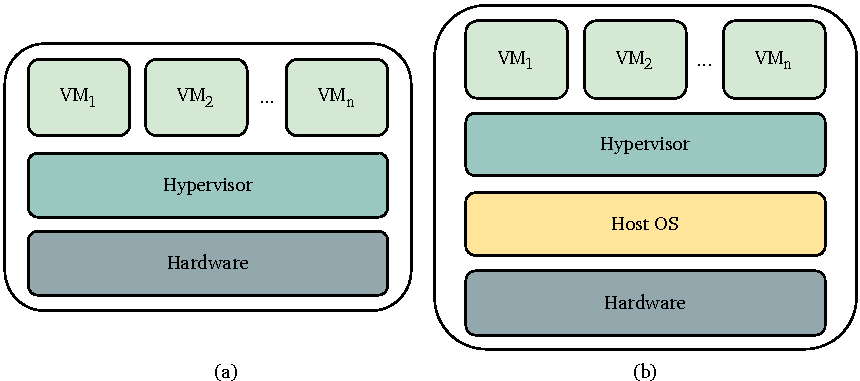
\includegraphics[width=1\textwidth]{figures/hypervisor.pdf}
    \caption{Two types of hypervisors including (a) Type-1 or Bare Metal hypervisor and (b) Type-2 or    Hosted hypervisor.}
    \label{fig24}
    \vspace{-8pt}
    \end{figure}
     \section{Hypervisor}
 
    %A hypervisor is a software layer that enables the creation and execution of virtual machines (VMs) on a physical host. A virtual machine is an emulation of a computer system that can run its own operating system and applications as if it were a physical computer. Hypervisors allow multiple virtual machines to share the hardware resources of a single physical host, enabling efficient use of hardware and reducing the need for multiple physical machines.There are two main types of hypervisors: type 1 (native or bare-metal) and type 2 (hosted).Type 1 hypervisors are installed directly on the physical host's hardware and manage the hardware resources, allowing multiple VMs to be created and run on the same physical host. Examples of type 1 hypervisors include VMware ESXi and Microsoft Hyper-V.Type 2 hypervisors are installed on top of a host operating system, which acts as a host for the VMs. Examples of type 2 hypervisors include VMware Workstation and Oracle VirtualBox.

    Hypervisors are commonly used in the automotive software domain to enable the development, testing, and deployment of software applications in a virtualized environment. This can reduce the cost and complexity of hardware infrastructure and provide a stable and isolated environment for testing and deploying applications. Moreover, hypervisors can be used to host multiple operating systems and applications on a single physical host, allowing for greater flexibility and scalability in deploying automotive software~\cite{9968908}.

    %The new software-defined architecture is an inseparable part of the future E/E architecture~\cite{shapiro2020future,askaripoor2022architecture}. Hardware virtualization technology should be taken into consideration to provide integration of safety and non-safety-critical software domains into the HPCU in such a way that does not violate the safety requirements and utilize the hardware resources as optimized as possible. This technology can be approached by using a hypervisor.A hypervisor is software that creates and executes virtual machines (VMs) so that the virtualized hardware resources will be shared among several instances using various types of OSs~\cite{dall2014kvm,askaripoor2022architecture,9968908}. 
    The emerging software-defined architecture plays an integral role in shaping the future E/E architecture~\cite{askaripoor2022architecture}. It is essential to consider hardware virtualization technology to seamlessly integrate safety-critical and non-safety-critical software domains into the HPCU while ensuring compliance with safety requirements and optimizing hardware resource utilization. This technology can be effectively implemented through a hypervisor, software designed to create and manage virtual machines (VMs). The hypervisor facilitates sharing virtualized hardware resources among multiple instances running various operating systems~\cite{askaripoor2022architecture,9968908}.
    There are two types of hypervisors:
   
    
    
    \begin{itemize}
    \item Type-1: %it is also called Bare Metal or Native hypervisor as it is installed and runs directly on top of the host's hardware without using any host OS. This type of hypervisor has direct control over and access to hardware resources. For example, a type-1 hypervisor can assign a specific core to a partition (an execution environment managed by the hypervisor which uses the virtualized services) in such a way that other partitions can not access that core~\cite{askaripoor2022architecture,9968908}.
    It is also known as the Bare Metal or Native hypervisor since it is installed and operates directly on the host's hardware without relying on any host operating system. According to Figure~\ref{fig24}~(a), this hypervisor possesses direct authority over and access to the hardware resources. For instance, a type-1 hypervisor can allocate a dedicated core to a partition (an execution environment supervised by the hypervisor that utilizes virtualized services) in a manner that prevents other partitions from accessing that core~\cite{askaripoor2022architecture,9968908}.
    
    
    \item Type-2: %it is also known as Hosted hypervisor. It runs as an application in the host OS and uses the hardware resources for its VMs by coordinating calls through the host's OS. The host OS does not have any knowledge about this type of hypervisor and it treats it like any other normal process~\cite{desai2013hypervisor}.
    It is also referred to as a Hosted hypervisor. This type of hypervisor operates as an application within the host OS and leverages hardware resources for its virtual machines (VMs) by directing requests through the host's OS based on Figure~\ref{fig24}~(b). Importantly, the host OS remains unaware of this hypervisor type, treating it like any other regular process~\cite{9968908,askaripoor2022architecture}.
    \end{itemize}
 
    The FFI requirement can be satisfied for safety-critical applications by using a hypervisor. For instance, based on the structure of the Bare Metal hypervisor presented in Figure~\ref{fig24}~(a), safety-critical applications can be run on VM$_1$. While QM applications can be executed on VM$_2$, ensuring that safety and non-safety-critical applications do not interfere with each other. 
    \begin{figure}[t]
    \centering
    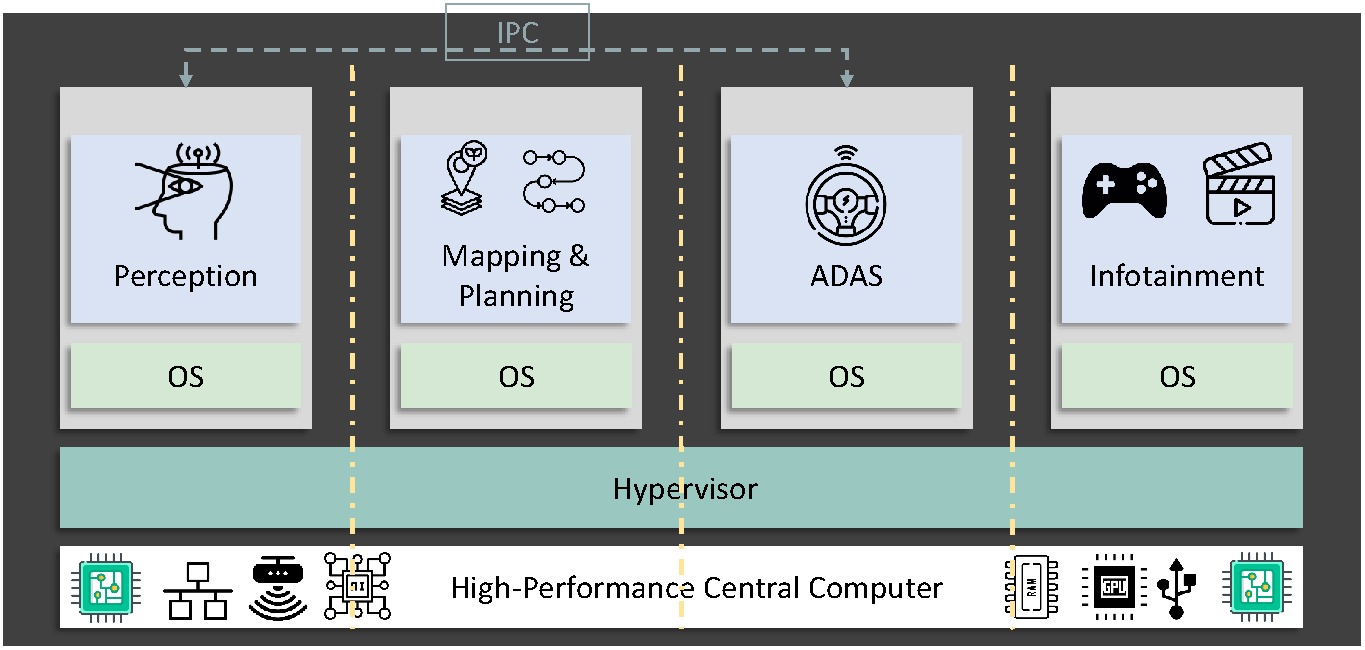
\includegraphics[width= \textwidth]{figures/hpcu_arch.pdf}
    \caption{The software architecture integrated into the vehicle's HPCU using a type-1 hypervisor consisting of four mixed-critical partitions. The yellow dash lines show the hard separations between partitions starting from the hardware level~\cite{askaripoor2022architecture}.}
    \label{fig012}
    \end{figure}
    Figure~\ref{fig012} illustrates a high-level software architecture for a vehicle integrated into a central HPCU. Different partitions are configured to isolate various application domains, including merging mixed-critical applications, to efficiently utilize hardware resources. This is achieved through the use of a type-1 hypervisor~\cite{9968908}, allowing each partition direct access to HPCU resources, such as cores, RAM, GPU, cache, network buses, and universal serial bus (USB) interfaces.
    As shown in Figure~\ref{fig012}, each partition operates with its OS and application domain, such as perception, layered on top of the OS. This arrangement ensures that each partition can utilize HPCU resources directly, thereby adhering to the principle of FFI as specified in ISO 26262~\cite{iso26262}. However, it is important to note that the extent to which resources follow the FFI requirement may vary depending on the choice of hypervisor. Various open-source and commercial hypervisors, developed by different companies, may offer different levels of FFI compliance based on the specific hardware configurations to be employed~\cite{askaripoor2022architecture}.
    
    In the context of the type-1 hypervisor, resources among partitions cannot be shared or accessed by other partitions, as indicated by the yellow dashed lines in Figure~\ref{fig012}~\cite{askaripoor2022architecture}.
    Furthermore, the inter-process communication (IPC) feature can activate communication between two partitions using a type-1 hypervisor. For example, suppose one process in a safety-critical partition (e.g., perception) intends to interact with another process in another (e.g., ADAS) to transfer messages. In that case, it can be accomplished by IPC (see Figure~\ref{fig012})~\cite{askaripoor2022architecture}.

    %\null
    %\addtocounter{page}{1}
    %\newpage
    %\thispagestyle{empty}
  

    
    
    \begin{comment}
    \section{Model Driven Development}
    Model-based system engineering
    \subsection{Software Integration and Configuration}
    Software integration and configuration in the design process for autonomous vehicles is the process of integrating and configuring the various software components that are necessary for the vehicle to function autonomously. This includes integrating and configuring the software for the sensors and perception systems that the vehicle uses to perceive its environment, as well as the software for the decision-making and control systems that allow the vehicle to navigate and make decisions on its own.
    
    In the design process for autonomous vehicles, software integration and configuration is a critical step because it ensures that all of the software components are working together seamlessly to enable the vehicle to function as intended. This process typically involves verifying that all of the software components are compatible with each other and that they are correctly configured to work together. It may also involve testing and debugging the software to ensure that it is functioning correctly and can handle a variety of different scenarios and conditions.
    
    Overall, software integration and configuration is a crucial part of the design process for autonomous vehicles because it ensures that the vehicle's software systems are properly integrated and configured, which is essential for the vehicle to operate safely and effectively in its environment.

%%%%%%%%%%%%%%%%%%%%%%%%%%%%%%%%%%%%another explanation%%%%%%%%%%%%%%%%%%%%%%%%%%%%%%

    Software integration and configuration are important steps in the design process for autonomous vehicles.
    
    Software integration involves combining different software components or systems into a cohesive whole, ensuring that they work together seamlessly. This can involve integrating different types of software, such as sensor processing software, decision-making software, and control software, as well as integrating software from different vendors or sources.
    
    Configuration refers to the process of setting up and tuning the software and hardware components of an autonomous vehicle to meet the specific requirements and performance goals of the system. This can involve configuring the vehicle's sensors and other hardware, as well as adjusting the software parameters and settings that control how the vehicle operates.
    
    Both software integration and configuration are critical to the successful design and deployment of autonomous vehicles. Ensuring that the various software and hardware components work together effectively and are properly configured is essential for ensuring the safety and reliability of the system.
    
    
    \subsection{E/E Architecture Synthesis and Design}
    Vehicle E/E architecture synthesis and design refers to the process of creating and implementing the electrical and electronic (E/E) systems and architecture for a vehicle. These systems and architecture include the hardware and software components that control and facilitate the functioning of the vehicle's various electrical and electronic systems, such as the powertrain, suspension, brakes, infotainment, and safety systems.
    
    The E/E architecture synthesis and design process typically involves several steps, including:
    
    Identifying and defining the requirements for the vehicle's E/E systems and architecture, including functional, performance, and safety requirements.
    
    Developing a conceptual design for the E/E architecture, including a top-level architecture diagram that shows the relationships between the various E/E systems and their interfaces.
    
    Defining the hardware and software components that will be used in the E/E architecture, including microcontrollers, sensors, actuators, and communication interfaces.
    
    Designing the electrical wiring and communication protocols that will be used to connect the various E/E components.
    
    Implementing and testing the E/E architecture, including writing the software code and integrating the hardware and software components.
    
    Validating the E/E architecture to ensure it meets all of the required functional, performance, and safety requirements.
    
    Maintaining and updating the E/E architecture throughout the vehicle's lifetime to ensure it continues to meet the changing needs of the vehicle.
    
    Overall, the goal of the vehicle E/E architecture synthesis and design process is to create a reliable, efficient, and safe E/E architecture that meets the needs of the vehicle and its users.

%%%%%%%%%%%%%%%%%%%%%%%%%%%%%%%%%%%%%%%%%Synthesis of Car E/E Architecture%%%%%%%%%%%%%%%%%%%%%%%%%%%%
    The synthesis of a car's electrical/electronic (E/E) architecture refers to the process of designing and integrating the various electrical and electronic systems that make up a modern automobile. This includes everything from the powertrain and drivetrain systems, to the infotainment and driver assist systems, as well as the various sensors, actuators, and controllers that enable these systems to function.
    
    To synthesize a car's E/E architecture, engineers must first identify the functional requirements of the vehicle and determine which systems and components are necessary to meet these requirements. This may involve conducting market research to understand consumer needs and preferences, as well as conducting simulations and prototypes to test and refine different design approaches.
    
    Once the functional requirements have been identified and the necessary systems and components have been selected, the next step is to design the overall architecture of the E/E systems. This involves determining the connections and interactions between the various systems and components, as well as designing the wiring and communication networks that will enable them to function together as a cohesive whole.
    
    Finally, the synthesis process involves integrating the various E/E systems and components into the car and testing them to ensure that they function as intended. This may involve extensive testing and debugging to ensure that the car's E/E architecture is reliable and performs to the desired specifications.




\subsection{Design Automation}
Design automation refers to the use of software tools and techniques to assist in the design and creation of electronic systems and devices. These tools can range from simple utilities that help with tasks such as layout and routing, to more advanced systems that can handle complex design tasks such as logic synthesis and verification.

The main goal of design automation is to improve the efficiency and effectiveness of the design process, by automating tasks that are time-consuming or error-prone when done manually. This can help to reduce design cycle times and improve the quality of the resulting designs.

There are many different types of design automation tools available, including computer-aided design (CAD) tools, simulation tools, and optimization tools. These tools can be used at different stages of the design process, from high-level architectural design to detailed implementation and verification.

Design automation is widely used in a variety of industries, including electronics, aerospace, automotive, and biomedical engineering. It is an important part of modern engineering practices and is constantly evolving as new technologies and design challenges emerge.

Design automation is the use of computer software and hardware tools to perform tasks related to the design and engineering of products or systems. It is a branch of engineering that focuses on the automation of design processes in order to increase efficiency, reduce errors, and accelerate time-to-market.

There are many different types of design automation tools, ranging from simple computer-aided design (CAD) software to more complex systems that can handle the entire design process from start to finish. Some common tasks that design automation tools can perform include:

Generating 3D models and 2D drawings of products or systems
Performing simulations and analysis to evaluate the performance of designs
Generating documentation and reports for regulatory or compliance purposes
Collaborating with other design tools or systems to exchange data and ensure consistency
Optimizing designs for cost, performance, or other criteria
Design automation can be applied to a wide range of industries, including manufacturing, automotive, aerospace, electronics, and many more. It is an essential part of modern product development and has significantly reduced the time and effort required to design and engineer complex systems.



\subsection{NP problems}

Furthermore, finding the correct schedules become an NP-hard problem as the size of the automotive network increases. 

NP (nondeterministic polynomial time) problems are a class of computational problems for which it is believed that no efficient solution (that is, an algorithm that can solve the problem in polynomial time) exists. These problems are considered to be some of the hardest problems to solve in computer science, and as a result, they have received a lot of attention from researchers.

In the context of scheduling and message routing, NP problems often involve finding the optimal or near-optimal solution to a problem with a large number of variables and constraints. Some examples of NP problems in this domain include:

Traveling salesman problem: Given a list of cities and the distances between them, find the shortest possible route that visits each city exactly once and returns to the starting city.

Resource-constrained project scheduling problem: Given a set of tasks with durations and resource requirements, and a set of resources with limited availability, find a schedule that completes all the tasks within a given time frame while minimizing resource usage.

Vehicle routing problem: Given a set of customers, each with a location and a demand, and a fleet of vehicles with limited capacity, find the least-cost route for the vehicles to follow in order to satisfy all the customer demands.

These problems are all NP-hard, which means that it is believed that there is no algorithm that can solve them in polynomial time. As a result, researchers have developed a variety of heuristics and approximation algorithms to find good (but not necessarily optimal) solutions to these problems.

%%%%%%%%%%%%%%%%%%%%%%%%%%%%%%time triggered scheduling%%%%%%%%%%%%%%%%%%%%%%%%%%%%%%%%%%%%%%%
Time-triggered scheduling is a method of scheduling tasks in real-time systems, in which tasks are executed at specific points in time (called "triggers") according to a predetermined schedule. This type of scheduling is used in systems where it is important to guarantee a certain level of predictability and determinism in the execution of tasks.

The problem of finding a schedule for a set of tasks in a time-triggered system is an NP problem because it involves finding a solution that satisfies a large number of constraints and minimizes some measure of cost or risk. In order to find an optimal schedule, it is necessary to consider all possible combinations of task assignments and trigger times, which can be very time-consuming.

One specific NP problem in the realm of time-triggered scheduling is the time-triggered scheduling problem with resource constraints (TTS-RC), which involves finding a schedule that meets the timing constraints of the tasks while also ensuring that the resource usage of the system does not exceed a certain threshold. This problem is NP-hard because it involves finding a solution that minimizes the cost of resource usage while satisfying all the timing constraints, which can be very difficult to do in polynomial time.

Overall, the complexity of time-triggered scheduling problems arises from the large number of variables and constraints involved, as well as the need to find a solution that satisfies a variety of conflicting objectives (such as minimizing resource usage while meeting timing constraints). These factors make it difficult to find an efficient algorithm for solving these problems, and as a result, they are considered to be NP problems.

%%%%%%%%%%%%%%%%%%%%%%%%%%%%%%%%%%%%%%%%%message routing%%%%%%%%%%%%%%%%%%%%%%%%%%%%%%%%%%%%%%%%%%%%%%
Message routing in communication refers to the process of finding the best path for a message to take from its source to its destination through a network of interconnected devices or nodes. In some cases, finding the optimal path for a message to take can be a computationally complex task, and it is possible to prove that certain types of message routing problems are NP-hard.

NP-hard problems are a class of problems in computer science that are believed to be difficult to solve. Specifically, an NP-hard problem is one for which it is believed that there is no known algorithm that can solve it in polynomial time (meaning, a time complexity of O($n^k$) for some constant k). Instead, solving an NP-hard problem typically requires exponential time (O($c^n$) for some constant c).

There are many different factors that can contribute to the complexity of message routing problems, including the size and structure of the network, the number of messages that need to be routed, and the constraints or objectives that need to be satisfied (such as minimizing the total distance traveled by the messages or maximizing the network's capacity). In some cases, finding the optimal solution to a message routing problem can require examining a large number of possible paths and comparing their relative costs or benefits, which can be computationally expensive.

Overall, message routing is a complex problem that can be difficult to solve efficiently, and it is possible to prove that certain types of message routing problems are NP-hard. However, there are also many practical techniques and heuristics that can be used to find good solutions to message routing problems in practice, even if they are not guaranteed to be optimal.
%\section{Safety Requirements}


    \end{comment}





\begin{comment}
\begin{figure}[t]
	\centering
	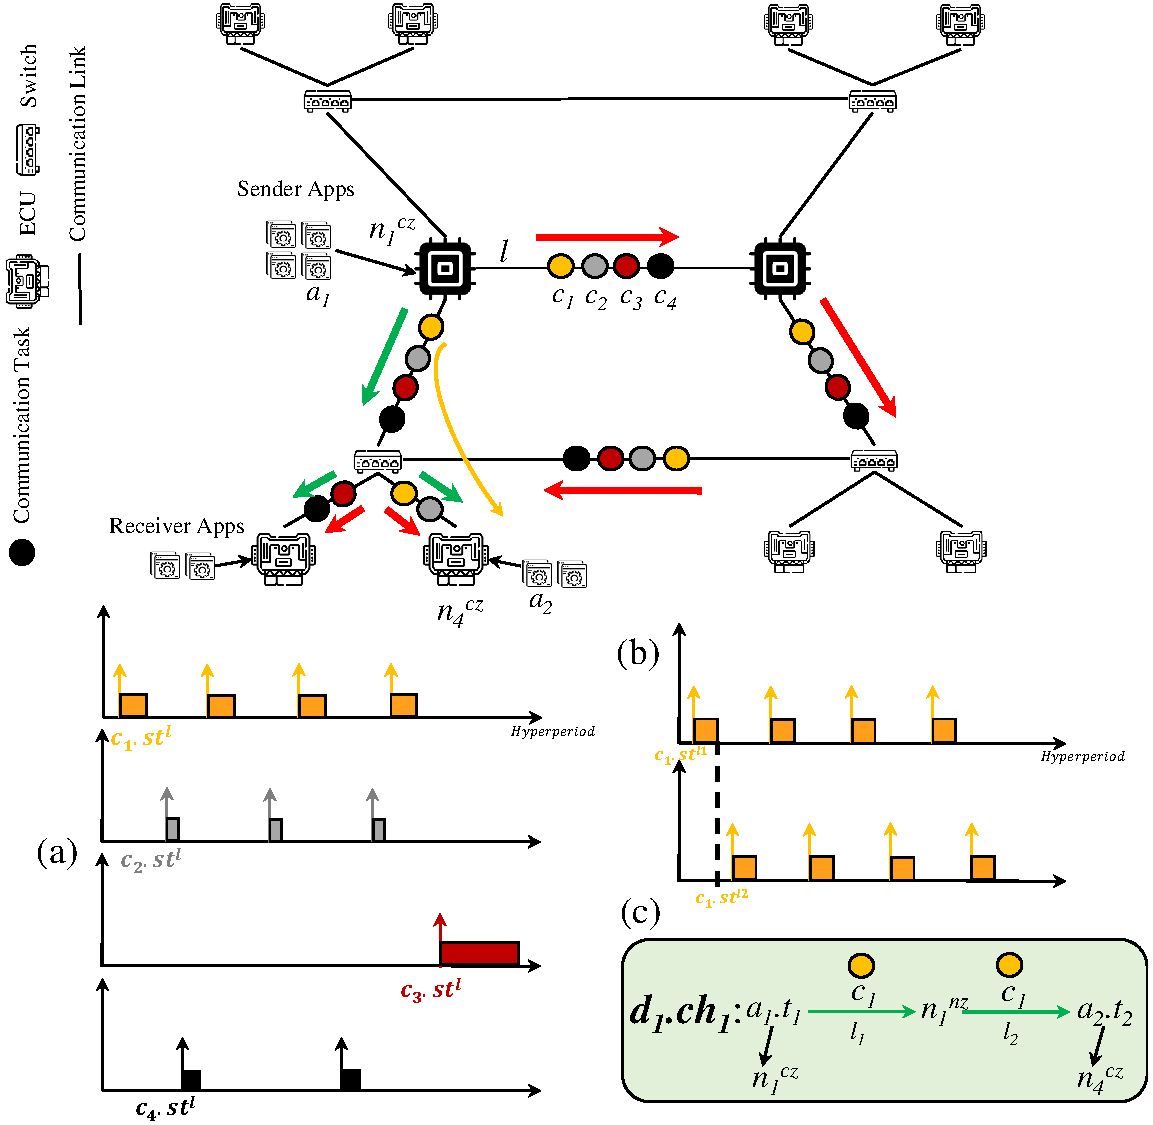
\includegraphics[width=1\columnwidth]{routing11.pdf}
	\caption{(a) Calculated time-triggered schedules for communication tasks including $c_1, c_2, c_3,$ and $c_4$ over $l$ link. 
	(b) Temporal order (Path Dependency) for $c_1$ task over green path (displayed with yellow arrow). (c) Task chain for communication message $d_1$ routing $c_1$ task from sender $t_1$ thread from $a_1$ to receiver $t_2$ from $a_2$ using green path.}
	\label{routing}
\end{figure}
\end{comment}


 
 
 %Furthermore, guaranteeing message transmission for safety-critical decisions. In addition, to enable real-time applications low latency and deterministic message delivery are required i.e., all computations must be completed before their respective deadlines. Therefore, a suitable communication protocol must be chosen to fulfill these requirements. There are various communication protocols like CAN, FlexRay, and Ethernet which offers higher bandwidth and latency requirements.  


 

    %\section{Design Space Exploration}
    
    %Design space exploration is a process in which different design alternatives are evaluated and compared in order to choose the best solution for a particular problem. This process typically involves identifying the design constraints and objectives, generating a set of possible design alternatives, and evaluating each alternative using a set of metrics or criteria. The ultimate goal of design space exploration is to identify the optimal design solution that meets the constraints and objectives of the problem while also being efficient, effective, and feasible to implement.There are many different techniques and approaches that can be used for design space exploration, depending on the specific problem and the design goals. Some common techniques include simulation, optimization, prototyping, and experimentation. The choice of technique will depend on the nature of the problem, the available resources, and the level of uncertainty involved in the design process.Design space exploration is an important part of the design process in many fields, including engineering, computer science, and product design. It allows designers to evaluate and compare different design alternatives in order to identify the best solution for a particular problem, and it helps to ensure that the final design is optimal and meets all of the necessary constraints and objectives.Design space exploration (DSE) is the process of evaluating different design alternatives in order to identify the most suitable solution to a design problem. It involves exploring different design options, analyzing their trade-offs, and selecting the best one based on a set of predefined criteria.DSE is commonly used in the field of computer engineering, where it is used to optimize the design of computer systems, circuits, and software. It can be applied at various levels of design abstraction, from the high-level specification of a system down to the detailed design of individual components.
    
    %DSE often involves the use of computational tools and techniques, such as computer-aided design (CAD) tools, simulation software, and optimization algorithms, to evaluate the performance and other characteristics of different design options. It may also involve experimentation and prototyping to verify the feasibility and effectiveness of a chosen design.The goal of DSE is to find a design that meets the specified requirements and constraints in the most efficient and effective way possible. It is an iterative process that may involve multi